%%%% --------------------------------------------------------------------------
%%
%%          K I L O N O V A
%%
%%%% --------------------------------------------------------------------------

\chapter{Kilonova} \label{ch:kilonova} 

In Sec.~\ref{sec:intro:kilonova} we discussed the thermal \ac{EM} 
counterpart to \ac{BNS} mergers, powered by the decay of newly 
synthesized heavy elements, \acl{kN} (\acs{kN}). 
%Now, having elaborated on the 
%\rproc{} yields in ejecta from our simulations (Chapter~\ref{ch:nucleo}), 
%we proceed with discussing the \ac{kN} light curves. 
In this Chapter we expand upon this discussion by computing 
\ac{kN} models for ejecta from our \ac{BNS} merger simulations, and comparing 
synthetic \acp{LC} to observations.
%
First, in Sec.~\ref{sec:kilonova:modeling} we overview the basic 
concepts behind modeling \ac{kN} emission. 
%, the energy release in nuclear heating, 
%its thermalization in ejecta, and the opacities of the latter and how 
%they shape the final emission giving a unique signature. 
%
Then, in Sec.~\ref{sec:kilonova:albino} we describe a particular model  
developed by \cite{Perego:2017wtu} that was used in our analysis 
to produce synthetic light curves. 
%
Finally, in Sec.~\ref{sec:kilonova:result} and Sec.~\ref{sec:kilonova:fitinformed}
we report the results of our analysis, and in 
Sec.~\ref{sec:kilonova:summary} we summarize the \ac{kN} signatures 
from different types of ejecta and compare them with \AT{}.

%% --------------------------
%% M O D E L L I N G  K I L O N O V A
%% --------------------------

%The \rproc{} \nuc{} in ejecta is primarily determined by the electron fraction 
%\citep{Lippuner:2015gwa}, $Y_e$, producing $3$rd ($1$st) elements of the \rproc{} peaks 
%%(See Sec.~\ref{sec:intro:nucleo}) 
%if the $Y_e\gtrsim 0.3$ ($Y_e \lesssim 0.2$) 
%with respective abundances in the former remarkably close to solar. 
%%The transition at $Y_e{\simeq}0.25$ is rather sharp.



\section{Overview of kilonova modeling} \label{sec:kilonova:modeling}

In general, ejecta from \ac{BNS} mergers is stratified and non-axisymmetric. 
A way to compute \ac{EM} emission from such ejecta is to perform 
multi-dimensional, 
multi-group radiative transfer simulations coupled to a \ac{HD} (or \ac{MHD}) 
simulation of ejecta itself. % \citep[\eg][]{Bulla:2019muo}.
%
It is, however, possible to compute bolometric\footnote{
    Related to the total emitted radiation at all wavelengths. 
} properties considering only the total amount 
of energy released and emitted by radioactive decay within the ejecta. 

%
%Here a simplified model is considered of a transient, powered by the radioactive decay 
%within the ejecta only. Several other assumptions are made. In particular, the ejecta 
%expansion is homologous (faster matter ahead of slow one) \citep{Rosswog:2013kqa}. %%{(Rosswog et al 2014)}
%
%\red{this is based on the Barnes PhD thesis on Opacities for Kilonva (Rad.Transport)}
%\red{Based on Metzger paper }

%% --------------------------
%% SIMPLE MODEL
%% --------------------------

%\subsubsection{Basic ingredients}

%Consider the following simplified approach to compute the \ac{EM} signal from \rproc{}
%elements enriched material. 
Let the radioactive decay of a newly synthesized heavy isotope, $i$, release 
$\dot{Q}_i \propto \exp(-t/\tau_i)$ energy, with $\tau_i$ being its half-life.
Then, assuming equal distribution of $\tau_i$ per logarithmic time, 
%(at any $t$ the dominant species have $\tau\sim t$), 
the heating rate of ejecta at time $t$ is 
$\dot{Q}_{LP} = f M c^2 / t$,
where $f$ is a free parameter and $M$ is the ejecta mass\footnote{
    In general, heating is time-dependent as thermodynamic histories of the expanding 
    ejecta (from \ac{NR} simulations) showed \citep{Metzger:2010,Roberts:2011,Korobkin:2012uy}.
    See also \citet{Hotokezaka:2017dbk} for the discussion on physical 
    principles behind the decay.
} \citep{Metzger:2019zeh}.
%
%In addition, provided by \citet{Li:1998bw}, normalization $f$ resulted in overestimation of the peak 
%luminosity of the \ac{kN}, that plagued the \ac{kN} searches for a decade 
%\cite{Rosswog:2005su,Dong:2015oea,Bloom:2005qx,Kocevski:2009gv}. 



%% ----------------------------------------
%\subsection{Basic model of the \ac{kN}}
%% ----------------------------------------

Then, for a single shell of hot and optically thick matter 
(in which the thermal energy is not immediately radiated away), 
and expanding with constant velocity, 
%such that $R\approx\upsilon t$ at any point in time $t$, 
the energy release 
%within the expanding ejecta 
can be described as follows.
For a shell of mass $\dd M_{\upsilon}$ and velocity $\upsilon$ that has a 
fraction of \rproc{} elements $X_{r,\upsilon}$, the energy release is 
given by the specific heating, $\dot{e}_r(t)$, and can be approximated as 
%
\begin{equation}
\dot{Q}_{r,\upsilon} = \dd M_{\upsilon}X_{r,\upsilon}\dot{e}_{r}(t).
\end{equation}
%

The optical depth $\tau$, and the 
radiation diffusion timescale $t_{\rm diff}$, are  
%
\begin{equation}
\tau = \rho \kappa R = \frac{3}{4}\frac{\dd M\kappa}{\pi R^2}, \hspace{5mm} 
t_{\rm diff} \approx \frac{R}{c}\tau = \frac{3}{4}\frac{\dd M\kappa}{\pi c R} = \frac{3}{4}\frac{\dd M\kappa}{\pi c \upsilon t}\, ,
\end{equation}
%
where 
%$M$ is the ejecta mass, 
$\kappa$ is the opacity (cross section per unit mass), and
$\rho$ is the mean density, \ie, $\rho=3 \dd M/(4\pi R^3)$.
%
As ejecta expands and cools (via adiabatic losses), its opacity decreases, 
and so does the diffusion timescale. 
When $t_{\rm diff}$ reaches $t$, the radiation can escape the ejecta \citep{Arnett:1982}. 
Hence, the characteristic timescale of the peak of the emitted radiation is 
%
%\red{check the eq.} -- Eq.5 in Metzger
\begin{equation}
t_{\rm peak} = \Big(\frac{3}{4\pi}\frac{1}{\beta}\frac{\dd M\kappa}{\upsilon c}\Big)^{1/2}\, ,
\end{equation}
%
where the constant $\beta$ depends on the exact ejecta density profile. 
The $t_{\rm peak}$ is of order of days for lanthanides-free and weeks for lanthanides-rich ejecta.
The peak luminosity is set by the total heating rate, $\dot{Q}(t)$, 
within the ejecta, as described by  \textit{Arnett's Law} 
\citep{Arnett:1982}. 

%% ----------------------------------------
%\subsubsection{Emission from stratified ejecta}
%% ----------------------------------------

%Consider the ejecta with a given mass-velocity distribution, that can be approximated 
%as $M_{\upsilon} = M(\upsilon / \upsilon_0)^{-\beta}$, for $\upsilon \geq \upsilon_0$,
%where $M$ is the total mass, $\upsilon_0$ is the average, minimum velocity. 
%The parameter $\beta$ can be set to $3$ \citep{Bauswein:2013yna}. %%{(Bauswein et al 2013a)}. 
%However see \citet{Piran:2012wd}%%{Piran et al 2013} 
%for a more complex velocity profiles.
%%
%%
%The diffusion timescale defines when the radiation escapes the ejecta. For a layer with 
%$\upsilon$ and $M_{\upsilon}$ and opacity $\kappa_{\upsilon}$ it is 
%%
%\begin{equation}
%t_{d,\upsilon} \approx \frac{3}{4\pi}\frac{M_{\upsilon}\kappa_{\upsilon}}{\beta Rc} = 
%\frac{1}{4\pi}\frac{M_{\upsilon}^{4/3}\kappa_{\upsilon}}{M^{1/3}\upsilon_0 t c}
%\end{equation}
%%
%where $\beta=3$ was assumed. 
%%
%This equation implies that at time $t=t_{d,\upsilon}$ the radiation from the layer 
%$M_{\upsilon}$ peaks.
%%
%The $M_{\upsilon}(t)$ is related to the total mass of the ejecta and 
%peak time (when radiation diffuses from the entire ejecta)
%%
%\begin{equation}
%M_{\upsilon}(t) = 
%\begin{cases}
%M(t/t_{peak})^{3/2},& t<t_{peak}, \\
%M, &t>t_{peak}
%\end{cases}
%\end{equation}
%%
%where $t_{peak} = (3M\kappa / (4\pi \beta \upsilon c))^{1/2}$ with 
%$\upsilon = \upsilon_0$. \red{Did not understand}
%%
%Outer layers with $M_{\upsilon} < M$ peak first, while the deepest layers peak later but 
%set the luminosity of the whole ejecta (assuming that the the opacity is constant in the 
%ejecta. 
%%
%The radial evolution of each layer $M_{\upsilon}$ of mass $dM_{\upsilon}$ is given by 
%%
%\begin{equation}
%\frac{dR}{dt} = \upsilon,
%\end{equation}
%%
%and the layer's thermal energy changes according to 
%%
%\begin{equation}
%\label{eq:theory:mkn:energ}
%\frac{dE_{\upsilon}}{dt} = \underbracket{-\frac{E_{\upsilon}}{R_{\upsilon}} 
%    \frac{dR_{\upsilon}}{dt}}_{PdV\text{ losses}} - 
%\underbracket{L_{\upsilon}}_{\text{rad. los.}} + \underbrace{\dot{Q}}_{\text{heating sources}},
%\end{equation}
%%
%where the radiative losses take form
%%
%\begin{equation}
%L_{\upsilon} = \frac{E_{\upsilon}}{t_{d,\upsilon} + t_{lc,\upsilon}},
%\end{equation}
%%
%in which the $t_{lc,\upsilon} = R_{\upsilon}/c$ limits the energy loss to the 
%light crossing time (important for when the layer is optically thin) \red{did not understand}.
%%
%The heating sources $\dot{Q}$ include
%%
%\begin{equation}
%\dot{Q}(t) = \underbrace{\dot{Q}_{r,\upsilon}}_{\text{radioactivity}} + \underbrace{\dot{Q}_{mag}}_{\text{magnetar}} + 
%\underbrace{\dot{Q}_{fb}}_{\text{fall-bak accretion}}.
%\end{equation}
%%
%%
%Next, even though in principle the effect of radiation pressure on ejecta oughtto 
%be considered, in case where radioactive heating, total energy input 
%$\int \dot{Q}_{r,\upsilon}dt < E_{kin,0}$ of the ejecta \citep{Metzger:2010,Rosswog:2013kqa} 
%%\cite{(Metzger et al 2011; Rosswog et al 2013)}, 
%this effect can be neglected.
%Meanwhile, central engine might provide enough energy to modify the free expansion 
%model. Then the equation for the central shell velocity evolution reads 
%%
%\begin{equation}
%\label{eq:theory:mkn:velcenteng}
%\frac{d}{dt}\Bigg(\frac{M\upsilon_0^2}{2}\Bigg) = M\upsilon_0\frac{d\upsilon_0}{dt} = \frac{E_{\upsilon_0}}{R_0}\frac{dR_0}{dt}
%\end{equation}
%%
%Here, the term with $E_{\upsilon_0}$ balances the $PdV$-\textit{loss} term in the 
%thermal energy equation (for $dE_{\upsilon}/dt$)
%%
%To compute the emitted radiation, first assume the black-body emission, 
%the thermal emission, with effective temperature 
%%
%\begin{equation}
%T_{eff} = \Bigg(\frac{L_{tot}}{4 \pi \sigma R_{ph}^2}\Bigg)^{1/4}
%\end{equation}
%%
%where $L_{tot} = \sum(L_{\upsilon dm_{\upsilon}})$ is the total luminosity 
%(cumulative for all mass shells). At the point where optical depth 
%$\sum(\kappa_{\upsilon}dm_{\upsilon})=1$ the photosphere is located with 
%radius $R_{ph}(t)$. 
%%
%%The flux density of the source at photon frequency $\nu$ is given by 
%%%
%%\begin{equation}
%%F_{\nu}(t) = \frac{2\pi h \nu^3}{c^2} \frac{1}{\exp\Big(\frac{h\nu}{kT_{eff}}\Big) - 1} \frac{R_{ph}^2}{D^2}
%%\end{equation}
%%%
%%where, $D$ is the distnace to the source. (Cosmological effects are neglected here).
%%
%Additionally, the opacity $\kappa_{\upsilon}$ depends on the temperature of the 
%layer $T_{\upsilon}$, that itself can be computed as 
%%
%\begin{equation}
%T_{\upsilon} = \Bigg(\frac{3E_{\upsilon}}{4\pi a R^{3}_{\upsilon}}\Bigg)^{1/4}
%\end{equation}
%%
%assuming that the ejecta internal energy is dominated by the radiation. 
%%
%%
%Finally, in order to compute the \ac{EM} emission from the ejecta, 
%the equation Eq.~\eqref{eq:theory:mkn:energ} ought be solved for $E_{\upsilon}$ 
%(and $L_{\upsilon}$) for every shell with $dM_{\upsilon}$ and $\upsilon>\upsilon_0$. 
%%
%The velocity distribution can be assumed fixed 
%(\eg $M_{\upsilon} = M(\upsilon/\upsilon_0)^{-\beta}$,  
%if only the internal heating are important. If however, the central engine energy 
%input is important, the the velocity of the central layer evolves according to
%Eq.~\eqref{eq:theory:mkn:velcenteng}.
%%
%Initial kinetic energy of the ejecta is quickly removed by the adiabatic expansion 
%and the thermal energy of the ejecta, when its emission peaks, is dominated by the heating.

%% -----------------
%% \paragraph{Opacity}
%% -----------------

% <<< MOVED TO INTRO 


%% ----------------------------
%% \paragraph{\rproc{} heating}
%% ----------------------------


%% <<< MOVED TO INTRO










%% =====================================================================================
%%
%%               I N T R O D U C T I O N
%%
%% =====================================================================================

\section{Semi-analytic kilonova model}\label{sec:kilonova:albino}

We compute the \ac{kN} light curves using a 
semi-analytic, multi-component, asnisotropic code \mkn{} 
\citep{Perego:2017wtu,Barbieri:2019sjc,Breschi:2021wzr}. 
%from the brief description of which we begin the chapter.
%
%Then we apply the code \mkn{} to the ejecta from our \ac{NR} \ac{BNS} 
%merger simulations and investigate how the newly found ejecta component, the 
%\ac{SWW} (see Ch.~\ref{ch:bns_sims}) affects the synthetic light curves and 
%compare the result with observations, the \AT{}.
%
The method can be summarized as follows. 


Each ejecta component (\eg, \ac{DE}, \ac{SWW}) is described through 
the angular distribution of its mass, $M_{\text{ej}}(\theta)$, 
velocity, $\upsilon_{\text{ej}}(\theta)$, and opacity, $\kappa_{\text{ej}}(\theta)$.
%
The polar angle, $\theta$, measured from the rotational axis of the \pmerg{} remnant, is discretized in 
$N_\theta=30$ angular bins evenly spaced in $\cos{(\theta)}$.
%
Additionally, within each ray, the matter has a fixed velocity distribution, 
$\xi(\upsilon) \propto (1 - (\upsilon / \upsilon_{\text{max}})^2)^3$,
%
%\begin{equation}
%\xi(\upsilon) \propto \Big(1 - \left(\frac{\upsilon}{\upsilon_{\text{max}}}\right)^{2}\Big)^{3}, 
%\end{equation}
%
where $\xi(\upsilon) \dd \upsilon$ is the matter contained in an infinitesimal layer of speed 
$\left[\upsilon,\upsilon+\dd \upsilon\right]$, and 
$\upsilon_{\text{max}}=\upsilon_{\text{max}}(\upsilon_{\text{RMS}})$ 
is the maximum velocity at the outermost edge of the ejecta component.
%
%The characteristic quantities are then evaluated for every bin according 
%to the assumed input profiles. 
%Then the emitted luminocity is evaluated for every bin 
%using the radial model described in \citet{Perego:2017wtu}, and in 
%\S{4} of \citet{Barbieri:2019kli}.


The emitted luminosity from every bin is evaluated according to the following model. 
%
The model assumes that the thermal radiation is emitted at the photosphere, located at 
$R_{\text{ph}}$, with effective emission temperature, $T_{\text{eff}}$, and 
is evaluated with the Stefan-Boltzmann law, \ie, assuming 
black-body radiation. This assumption is justified 
for modeling the early emission when ejecta is hot and opaque. 
%However, at later 
%times, as ejecta falls out of \ac{LTE} with its radiation, the assumption breaks.
%
%%%% -----------------------
% Heating rates
%%%% -----------------------
%The time-dependent nuclear heating are approximated as Eq.~\eqref{eq:kilonova:eps_korob}.
%rate $\epsilon_{\text{nuc}}$ \red{assert notations} entering these calculations is approximated 
%by an analytic fitting formula, derived from detailed nucleosynthesis 
%calculations~\citep{Korobkin:2012uy} Eq.~\eqref{eq:kilonova:heat_korob}, 
%modified as follows
%                                            << moved above >>>
%\begin{equation}
%\label{eq:epsnuc}
%\epsilon_{\text{nuc}}(t)= \epsilon_0 \, \frac{\epsilon_{\text{th}}(t)}{0.5} \, \epsilon_{\text{nr}}(t) \,
%\left[ \frac{1}{2} - \frac{1}{\pi} \arctan\left(\frac{t-t_0}{\sigma}\right)\right]^{\alpha}\,,
%\end{equation}
%%
%where $\sigma = 0.11$~s, $t_0 = 1.3$~s, $\alpha=1.3$ and $\epsilon_{\text{th}}(t)$ is the 
%thermalization efficiency tabulated according to \citet{Barnes:2016umi}.
%\red{$\epsilon_0$ is not introduced. Is it a constant?}
%%
%The heating factor $\epsilon_{\text{nr}}(t) $ is introduced as in \citet{Perego:2017wtu} to roughly adjust 
%the Eq.~\eqref{eq:epsnuc} in the regime of mildly neutron-rich matter (characterized by an initial 
%electron fraction $Y_e \gtrsim 0.25$), \citep[see, \eg][]{Martin:2015hxa}:
%%
%\begin{equation}
%\label{eq:epsnr}
%\epsilon_{\text{nr}}(t,\kappa) = \left[1-w(\kappa)\right] + w(\kappa)\,\epsilon_{Y_e}(t)\,,  
%\end{equation}
%%
%where $w(\kappa)$ is a logarithmic smooth clump function such that $w(\kappa < 1~\igscm) = 1$ and 
%$w(\kappa > 10~\igscm)=0$ and the factor $\epsilon_{Y_e}(t)$ accounts for the dependency on $Y_e$:
%if $Y_e < 0.25$, then $\epsilon_{Y_e}(t)=1$, otherwise, when $Y_e \ge 0.25$,
%%
%\begin{equation}
%\label{eq:epsye}
%\epsilon_{Y_e}(t) =\epsilon_{\text{min}}+{\epsilon_{\text{max}}}{\left[1+ e ^{4(t/t_\epsilon-1)}\right]}^{-1}\,,
%\end{equation}
%%
%where $t_\epsilon = 1~{\text{day}}$, $\epsilon_{\text{min}}=0.5$ an $\epsilon_{\text{max}} = 2.5$.


%% FROM Breschi et al (from perego et al)

Time-dependent nuclear heating rates, $\epsilon_{\text{nuc}}$, 
%\red{assert notations} 
are approximated via an analytic fitting formula, derived from detailed 
nucleosynthesis calculations~\citep{Korobkin:2012uy}  
%
\begin{equation}
\label{eq:kilonova:eps_korob}
\epsilon_{\text{nuc}}(t)= \epsilon_0 \, \frac{\epsilon_{\text{th}}(t)}{0.5} \, \epsilon_{\text{nr}}(t) \,
\left[ \frac{1}{2} - \frac{1}{\pi} \arctan\left(\frac{t-t_0}{\sigma}\right)\right]^{\alpha}\,,
\end{equation}
%
where $\sigma = 0.11\,$s, $t_0 = 1.3\,$s, $\alpha=1.3$,
$\epsilon_0$ is the constant and 
$\epsilon_{\text{th}}(t)$ is the 
thermalization efficiency, tabulated according to \citet{Barnes:2016umi}.
%
For a neutron-rich ejecta, $Y_e\leq 0.2$, the heating rate is dominated by a large statistical 
ensemble of nuclei, however, at higher $Y_e\gtrsim 0.2$, corrections are required. 
%
These corrections are introduced in a form of time-dependent heating factor, 
$\epsilon_{\text{nr}}(t)$, adjusted 
roughly to the regime of mildly neutron-rich matter \citep{Perego:2017wtu}. 

%The heating factor $\epsilon_{\text{nr}}(t) $ is introduced as in \citet{Perego:2017wtu} 
%to roughly adjust the Eq.~\eqref{eq:kilonova:eps_korob} tp the regime of mildly 
%neutron-rich matter (characterized by an initial electron fraction $Y_e \gtrsim 0.25$), 
%\citep[see, \eg][]{Martin:2015hxa}. 
%
%\begin{equation}
%\label{eq:epsnr}
%\epsilon_{\text{nr}}(t,\kappa) = \left[1-w(\kappa)\right] + w(\kappa)\,\epsilon_{Y_e}(t)\,,  
%\end{equation}
%%
%where $w(\kappa)$ is a logarithmic smooth clump function such that $w(\kappa < 1~\igscm) = 1$ and 
%$w(\kappa > 10~\igscm)=0$ and the factor $\epsilon_{Y_e}(t)$ accounts for the dependency on $Y_e$:
%if $Y_e < 0.25$, then $\epsilon_{Y_e}(t)=1$, otherwise, when $Y_e \ge 0.25$,
%%
%\begin{equation}
%\label{eq:epsye}
%\epsilon_{Y_e}(t) =\epsilon_{\text{min}}+{\epsilon_{\text{max}}}{\left[1+ e ^{4(t/t_\epsilon-1)}\right]}^{-1}\,,
%\end{equation}
%%
%where $t_\epsilon = 1~{\text{day}}$, $\epsilon_{\text{min}}=0.5$ an $\epsilon_{\text{max}} = 2.5$.

%%%% --------------
% Opacity 
%%%% --------------
%
The mean plank opacities for the hot ejecta are adopted from the recent systematic study by \citet{Tanaka:2019iqp}.
%Notably, the atomic opacity depends on its ionization state. %\red{might reference Barns work}.
Notably, when ejecta  temperature drops and atoms become neutral, 
the photon opacity sharply decreases. 
This was shown to have a strong effect on \acp{LC} in high-frequency bands 
%\eg, $V$, $U$, $B$ and $g$ 
\citep{Villar:2017oya}. In order to account 
for the drop in opacity when the temperature falls below a certain value,
corresponding to the full 
recombination, the $T_{\text{floor}}$ is introduced  
as a minimum value that $T_{\text{eff}}$ can have \citep{Kasen:2017sxr,Kasen:2018drm}. 
Because \ac{BNS} merger ejecta composition can include a significant amount of lanthinides, 
\texttt{MKN} employs two floor temperatures 
depending on the composition: the $T_{\text{floot}}^{\text{Ni}}$ and 
$T_{\text{floot}}^{\text{La}}$ for lanthanides free and rich ejecta, respectively.



%----  EATS integrator
The emission coming from different angular bins is combined to obtain the 
spectral flux at the observer location as, 
%
\begin{equation}
\label{eq:spectral_flux}
F_{\nu}(\mathbf{n},t) = \int_{\mathbf{n}_{\Omega} \cdot \mathbf{n}> 0} 
\left( \frac{R_{\text{ph}}(\Omega,t)}{D_L} \right)^2  B_{\nu}(T_{\text{eff}}(\Omega,t))~\mathbf{n} \cdot  \dd\boldsymbol{\Omega}\, , 
\end{equation}
%
where $\mathbf{n}$ is the unitary vector along the line of sight, 
$\mathbf{n}_{\Omega}$ is the unitary vector spanning the solid angle 
$\Omega$, $D_L$ is the luminosity distance, $R_{\text{ph}}$ is the local 
radial coordinate of the photospheric surface, and $B_{\nu}(T_{\rm eff})$ 
is the spectral radiance at frequency $\nu$ for a surface with temperature $T_{\text{eff}}$. 
%
% ---- Magnitudes
We also make use of the apparent AB magnitude, mag$_b$, 
in a given photometric band, $b$, defined as:
%
\begin{equation}
\label{eq:mag}
\text{mag}_b(\mathbf{n},t) = -2.5 \log_{10}\left( F_{\nu_b}(\mathbf{n},t) \right)-48.6\,,
\end{equation}
where $\nu_b$ is the effective central frequency of the band $b$.

%\begin{figure}
%    \centering 
%    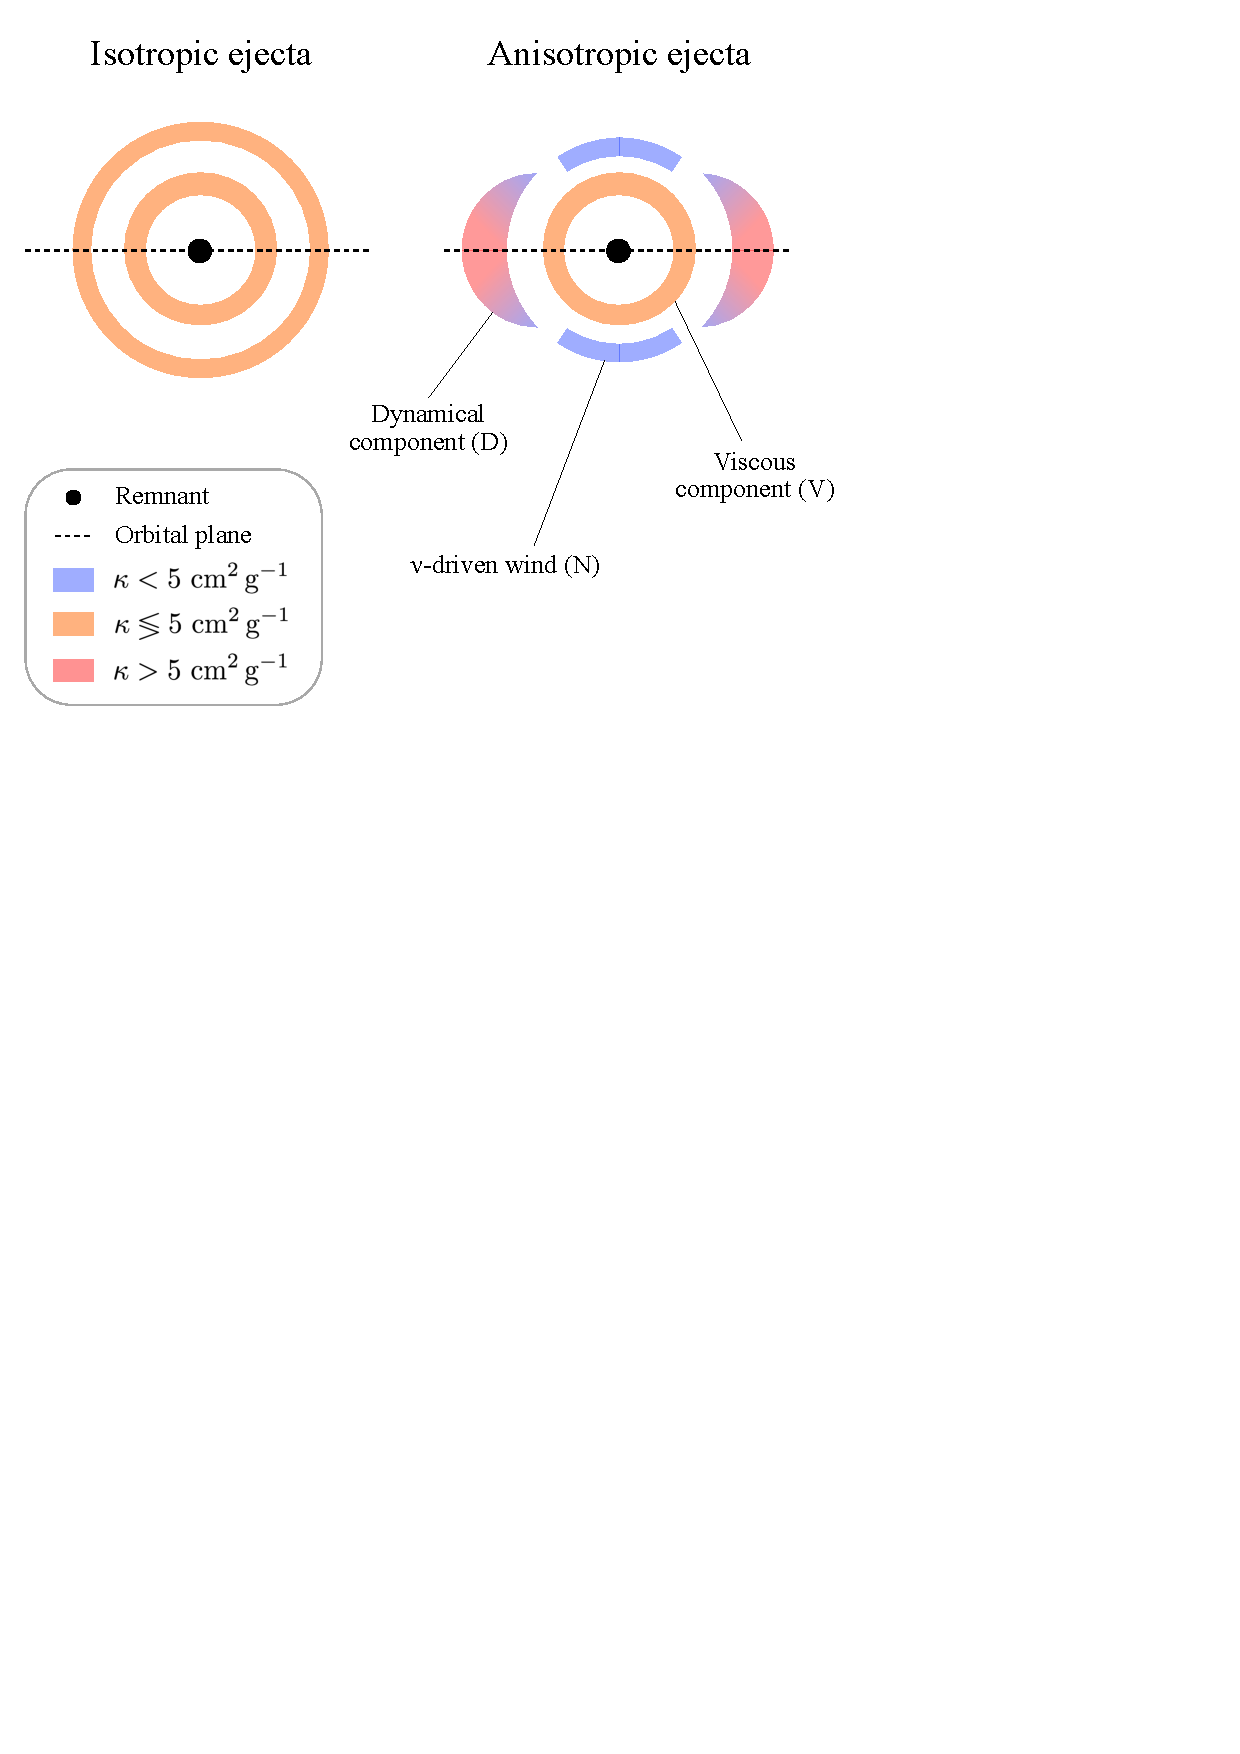
\includegraphics[width=0.58\textwidth]{profiles_op.pdf}
%    \caption{
%        Schematic representation of different ejecta components, comparing two 
%        cases: isotropic and anisotropic. 
%        In the former, the ejecta properties 
%        do not had angular dependency (uniform colors). In the latter, the 
%        different ejecta components are allowed to have different angular distribution 
%        of its properties, \eg, \ac{DE} confined to the plane of the binary and 
%        polar, low-opacity, \nwind{}.
%        Colors indicates the optical opacity, increasing from blue to red. 
%        %        Graphic representation of the analyzed
%        %        ejecta profiles for isotropic and anisotropic cases
%        %        from an azimuthal perspective and for a fixed moment of time.
%        %        The black dot represents the remnant and the dashed line is the projected orbital
%        %        plane of the binary. The shadowed areas describe the ejecta profiles: the shape
%        %        characterizes the mass distribution, while the colors refer to 
%        %        the prior assumptions on the opacity parameter.
%        %        In particular, blue regions denote opacities lower than $5~\igscm$,
%        %        red regions refer to opacities greater than $5~\igscm$,
%        %        and oranges areas indicate a broadly distributed opacity.
%        %        All shells are isotropically expanding with a constant velocity.
%        (Adapted from \citet{Breschi:2021wzr})
%    }
%    \label{fig:cartoon}
%\end{figure}




We consider \ac{DE} ejecta and \ac{SWW} geometries directly imported from 
our \ac{BNS} merger simulations in a form of angular profiles 
(assuming axisymmetry). We refer to such \ac{kN} models as \ac{NR}-informed. 
%with 
%respect to the polar angle and averaging over the azimuthal angle.
In several cases we also use analytical ejecta profiles, with 
either smooth or step-like dependency on the polar angle.
%
The viewing angle, $\theta_{\text{obs}}$, is measured as the angle between the 
polar axis and the \ac{LOS} of the observer.












%% =====================================================================================
%%
%%               R E S U L T S
%%
%% =====================================================================================

%In the following we perform two types of the analysis (i) the fully \ac{NR}-informed \ac{kN} models, where the the only ejecta components considered, are those found in simulations and (ii) the parametric \ac{kN} models, where we use the analytic ejecta profiles, with the parameters obtained from fitting formulae (see Ch.~\ref{ch:stat_anal}).

\begin{figure}[t]
    \centering
    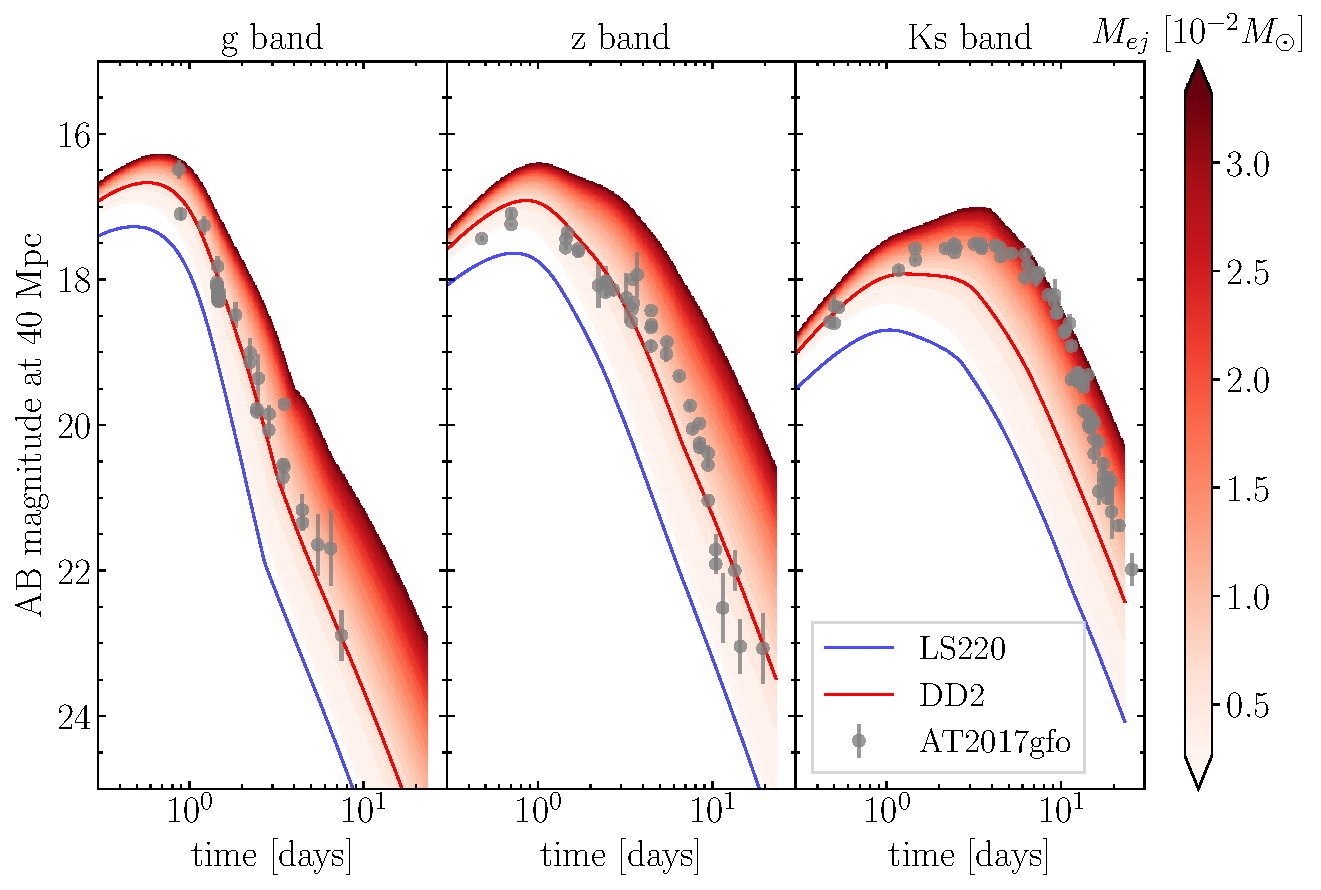
\includegraphics[width=0.80\textwidth]{kilonova/mkn_dd2_band.pdf}
    \caption{
        Bolometric \acp{LC} in three photometric bands (one per panel) for 
        ejecta from two \ac{BNS} merger models, 
        DD2 $q=1.00$ and LS220 $q=1.00$. \acp{LC} corresponding to 
        \ac{DE} only are shown with solid lines, while the red color gradient 
        represents a range of possible \acp{LC} for \ac{DE} plus \ac{SWW}, 
        depending on the total mass of the latter (color-coded). 
        The \ac{SWW} mass flux for DD2 $q=1.00$ is linearly extrapolated 
        after the end of the simulation until $250\,$ms \pmerg{}.
%        \ac{DE} (solid lines) and \ac{DE} plus 
%        \ac{SWW} (color gradient)
%        
%        Bolometric kN light curves in three representative bands from blue to
%        infrared for the two simulations with turbulence viscosity compared to
%        \AT{} data from~\citep{Villar:2017wcc}.
%        The color gradient is the effect related to different
%        \ac{SWW} masses, that suggests possible variations of the light
%        curves for different \ac{BNS}. The band is computed by extracting the
%        \ac{SWW} mass from DD2 every $10$~ms until the end of the simulation, and
%        then by linearly extrapolating the data to $250$~ms.
%        (Adapted from \citet{Nedora:2019jhl})
    }
    \label{fig:knlc}
\end{figure}





%\section{\ac{SWW} for the blue component of \AT{}}\label{sec:kilonova:result}
\section{Numerical relativity informed kilonova models}\label{sec:kilonova:result}
%The \ac{BNS} merger ejecta consists of several anisotropic components with different 
%properties (see the discussion in Sec.~\ref{sec:intro:ejecta} and Chapter~\ref{ch:bns_sims}).
%
%Hence, the \ac{kN} model ought to account for the anisotropy of the ejecta composition. Additionally, the interaction between components needs to be included, but we leave this to future works.
%% ---
%The outflow properties inferred for \AT{} using multi-components and 
%2D \ac{kN} models including the ejecta anisotropy and cross-component 
%irradiation are broadly compatible with the results from simulations, \eg,  \citep{Kawaguchi:2018ptg}.% see also Sec.~\ref{sec:intro:kilonova}. 
%%% ---
%The particular challenge however, is to reproduce the early blue emission. 
%Both semi-analytical and radiation transport models require ejecta properties 
%different from those found in simulations. In particular, this component 
%requires fast low opacity, massive ejecta \citep{Fahlman:2018llv} that is generally 
%not found in \ac{BNS} simulations.
%%% ---
%Notably, the early blue component can be explained by the emission arising 
%in the interaction between a relativistic jet and the ejecta
%\citep{Lazzati:2016yxl,Bromberg:2017crh,Piro:2017ayh}.
%However, simulations show that that successful jets do not deposit a sufficient amount of thermal energy in the ejecta for this mechanism to work \citep{Duffell:2018iig}. 
%Other possibilities include the presence of highly magnetized winds \citep{Metzger:2018uni,Fernandez:2018kax},
%or the presence of the so-called viscous dynamical ejecta \citep{Radice:2018ghv}.
%These two explanations require the development of large-scale strong magnetic fields.
%% ---
%In Sec.~\ref{sec:intro:kilonova} we mentioned that one of the still open 
%questions with regards to \AT{} is the origin of the early blue emission. 
%%
%In this section we show that the presence of the massive \ac{SWW},
%found in the ab-initio \ac{BNS} merger simulations with long-lived \ac{NS} remnants 
%(see Chapter~\ref{ch:bns_sims}) provides a tentative explanation for it, 
%%explain the early blue emission, 
%relaxing the need for strong ordered magnetic fields. 






We begin by considering two equal mass \ac{BNS} merger models with LS220 
and DD2 \acp{EOS}, that produce short and long-lived \pmerg{} remnants respectively
(see Chapter~\ref{ch:bns_sims}). 
Using the \texttt{MKN} code, discussed above, we compute \ac{NR}-informed 
\acp{LC} for both \ac{DE} only, and the combination of \ac{DE} and \ac{SWW}\footnote{
    The \texttt{MKN} code does not include the effects of ejecta component 
    iteration. We leave this to future works.
}. 
%%% ---
%For both models we produce \ac{NR}-informed \acp{LC}, using both the \ac{DE} and \ac{SWW} for the model with the long-lived \ac{MNS} remnant, and \ac{DE} only for the model with the short-lived one.
%% ---
The result is shown in Fig.~\ref{fig:knlc}. We observe that
%between the two \ac{BNS} models, 
when only \ac{DE} is considered, the \ac{kN} emission is 
significantly dimmer in the case of the LS220 $q=1.00$ model.
%
And while the amount of mass ejected by both models is rather similar,  
\ac{DE} from the DD2 $q=1.00$ model is faster and less neutron-rich, and hence 
have lower photon opacities. 

However, \ac{DE} alone do not produce emission bright enough to 
match \AT{}, especially at early times in $g$ band and at late times in $K_s$ band. 
The latter can be attributed to the absence of low-$Y_e$ secular ejecta in 
our simulations. 
%(see Sec.~\ref{sec:intro:kilonova}). 
The former, however, 
suggests the need of a low-$Y_e$, massive ejecta component. 
%
It is natural to consider whether \ac{SWW} can account for this early 
blue emission. Since the total mass of \ac{SWW} depends on the 
lifetime of a remnant, $t_{\rm coll}$, (see Sec.~\ref{sec:bns_sims:sww}) 
and the remnant of the DD2 $q=1.00$ model does not collapse until the end of 
the simulation (${\sim}100\,$ms \pmerg{}), we extrapolate the \ac{SWW} mass, 
considering a range of $t_{\rm coll}$ up to $250\,$ms \pmerg{}. The range of 
associated \ac{kN} \acp{LC} is shown in Fig.~\ref{fig:knlc} as red color gradient. 
%
The analysis suggests that sufficiently massive \ac{SWW} can indeed 
account for the early blue emission of \AT{}. However, the emission 
in other bands, \eg, $z$ band, becomes significantly brighter than 
what was observed. 

Our results, however, have uncertainties related to our simplified calculation 
of \ac{kN} \acp{LC} which is expected to be less accurate at late times when 
absorption features and deviations from \ac{LTE} become more relevant 
\citep[see \eg][]{Smartt:2017fuw}. 
%
A more detailed analysis of \acp{kN} produced by \ac{DE} and \ac{SWW}, that 
considers various ejecta profiles and cross-ejecta interactions, dynamical as 
well as radiative, is required to draw a more solid conclusion. 
%
%The result is shown in Fig.~\ref{fig:knlc}. 
%We observe, that emission from \ac{DE} alone cannot explain \AT{} in 
%all bands irrespective of the \ac{BNS} model. However, the informed 
%by both \ac{DE} and \ac{SWW} \ac{LC} of the DD2 $q=1.00$ model 
%is sufficiently bright to account for the emission in 'z' band. 
%%% However, it appears dimmer than the early blue \AT{} emission in 'g' band. 
%%% ---
%The emission in low frequency bands requires a more massive 
%\ac{SWW} with mass ${\gtrsim} 2\times10^{-2}M_{\odot}$, implying a remnant lifetime of ${\gtrsim}200$~ms, as the \ac{SWW} mass flux is present as long 
%as \ac{MNS} remnant is present (see Sec.\ref{sec:bns_sims:mj_loss}).
%However, a more massive \ac{SWW} is incompatible with
%the early emission for the low-frequency bands of \AT{}.
%%% --- 
%In order to explain the late emission in the low frequncy bands and 
%early emission in high frequency bands, a combination of the \ac{SWW} and 
%viscous ejecta from the disintegration of the disk are required.
%% --- 

%Additionally results, however, have uncertainties related to our simplified calculation of
%\ac{kN} \acp{LC} which is expected to be less accurate at late times when absorption 
%features and deviations from \ac{LTE} become more relevant \citep[see \eg][]{Smartt:2017fuw}.
%
%To model the \ac{kN} emission more robustly, the time- and energy-dependent 
%photon radiation transport models are required 
%\citep{Kasen:2017sxr,Tanaka:2017qxj,Miller:2019dpt,Bulla:2019muo}.
%Additionally, the systematic uncertainties in
%nuclear (\eg, mass models, fission fragments and $\beta$-decay
%rates) and atomic (\eg, detailed wavelength dependent opacities for
%\rproc{} element) physics enter all the current \ac{kN} models 
%\citep{Eichler:2014kma,Rosswog:2016dhy,Gaigalas:2019ptx}.

%% KILONVA PLOTS
\begin{figure*}[t!]
    \centering 
    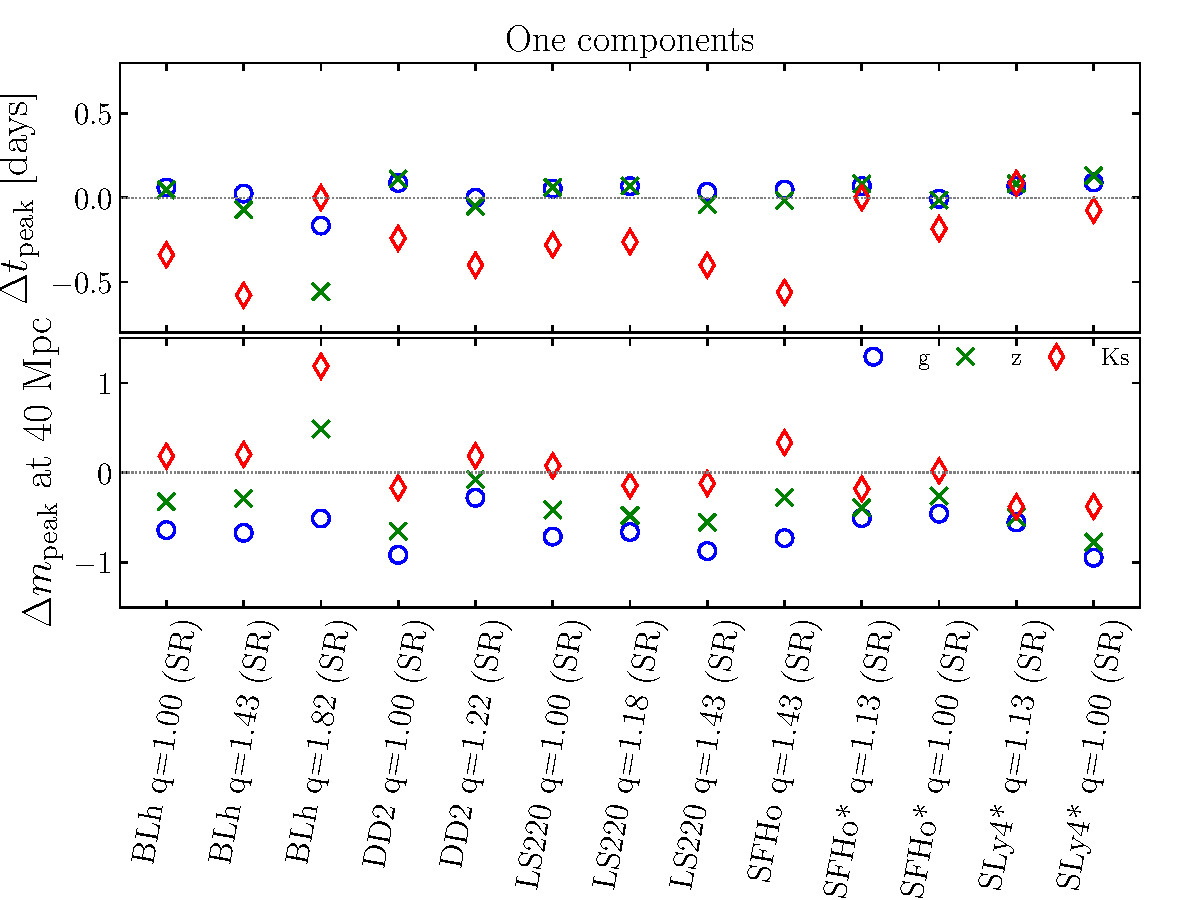
\includegraphics[width=0.72\textwidth]{kilonova/mkn_multiband_dyn_res_NR.pdf}
    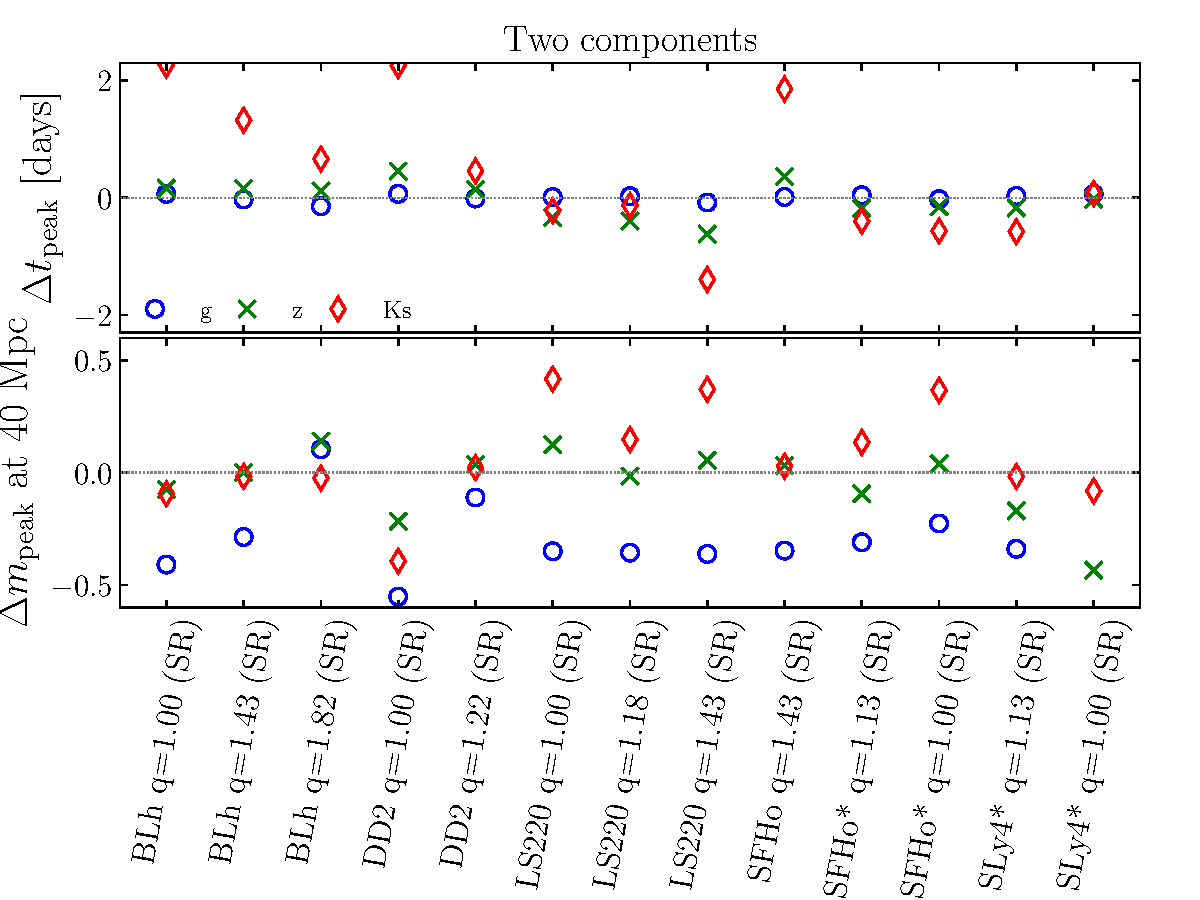
\includegraphics[width=0.72\textwidth]{kilonova/mkn_multiband_dynsec_res_NR.pdf}
    \caption{
        Differences in peak time (\textit{top subpanel}) and peak magnitude 
        \textit{(bottom subpanel)} between fit-informed \ac{kN} model \acp{LC}, 
        and \acp{LC} computed using the actual ejecta profile from a simulation. 
        %
        The \textit{top panel} shows this comparison for a single component \ac{kN} model 
        (only considering \ac{DE}), while the \textit{bottom panel} is for two-component 
        model, where \ac{DE} and secular winds are considered.
        %
        The comparison is shown for three different bands indicated with different markers.
        %
        The best result is when all three markers of all three colors are at $0$ for a 
        given simulation.
        %        Comparison between one component light curves (\textit{left panel}) and
        %        two components light curves (\textit{right panel}) in $g$, $z$ and $K_s$
        %        bands using direct NR input or the fitting formulae for the
        %        dynamical ejecta and disk mass. 
        %        The $y-$axis displays the difference between the peak time 
        %        (\textit{top panel}), $\Delta t_{\rm peak} = t_{\rm peak; NR} - t_{\rm peak; fit}$, 
        %        and peak magnitude, $\Delta m_{\rm peak} = m_{\rm peak; NR} - m_{\rm peak; fit}$, 
        %        (\textit{bottom panel});
        %        the $x-$axis shows selected BNS models of \DSrefset{}.
        %        The fits employed here are the polynomials in $(q,\tilde{\Lambda})$ used with the 
        %        best fitting coefficients, calibrated to \DSheatcool{} (that includes \DSrefset{}).
        %        The plot shows that 
        %        the light curves generated with the dynamical ejecta fits (one
        %        component) tend to underestimate the peak times and magnitudes
        %        of NR-informed light curves, especially in the $K_s$ band. In case of 
        %        dynamical ejecta and disk wind (two
        %        components) light curves, the peak
        %        time is less constrained ($\pm 2$~days) in the $K_s$ band, but the
        %        peak magnitudes is predicted more accurately $\pm0.5$~mag.
    }
    %% \vn{Note! That for NR-informed lightcurves \textbf{full} NR ejecta profile (for dyn. ej.)
    %% is fed into MKN. Thus here the geometric effects and poor fit performance contribute to the
    %% qdeviation.}
    \label{fig:mkn_example}
\end{figure*}


%\subsection{Conclusion}
%
%\red{Copied}
%Standard kN models applied to the early AT2017gfo light curve are in
%tension with ab-initio simulations conducted so far.
%While alternative interpretations have been proposed, they are either
%disfavored by current simulations and observations (e.g. jets) \citep{Bromberg:2017crh,Duffell:2018iig},
%or require the presence of large-scale strong magnetic 
%fields which might not be formed in the postmerger
%\citep{Metzger:2018uni,Fernandez:2018kax,Radice:2018ghv,Ciolfi:2019fie}. 
%We identified a robust dynamical mechanism for mass ejection that
%explains early-time observations without requiring any fine-tuning.
%The resulting nucleosynthesis is complete and produces all
%$r$-process elements in proportions similar to solar system abundances.
%Methodologically, our work underlines the importance of employing
%NR-informed ejecta for the fitting of light-curves.
%Further work in this direction should 
%include better neutrino-radiation transport and magnetohydrodynamic effects
%\citep{Siegel:2017nub,Fujibayashi:2017puw,Radice:2018xqa,Radice:2018pdn,Miller:2019dpt}. 


\section{Fit-informed kilonova models}\label{sec:kilonova:fitinformed}




%In this section we investigated statistical properties of the \ac{DE} and remnant from 
%several sets of \ac{NR} \ac{BNS} models. 
%
%The analysis showed that the properties of the ejecta and remnant disk mass are subjected 
%to large systematic uncertainties that stem from difference in input physics: neutrino 
%treatment and \ac{EOS}.
%%
%Additionally, we assessed the performance of different fitting formulae to the ejecta 
%parameters, such as mass, velocity, electron fraction and \ac{RMS} half-opening angle, 
%and the disk mass. We noted that the formulae that include explicitly $\tilde{\Lambda}$ 
%and \mr{} are able to capture the leading trends. Specifically, the simple second order 
%polynomial, $P_2^2(q,\tilde{\Lambda})$ performs on par or better than more complex 
%fitting formulae in terms of $\chid$.
%%
%However, all fits are characterized by large $\chid$. That suggests that either the 
%error measures we adopt are too strict, or more complex fitting formulae are required. 
%We leave this investigation to future works, when larger sample of \ac{NR} \ac{BNS} 
%models with advanced physics is available.
%%
%%We stress that while these fits, provide an important links between the binary parameters 
%%and the properties of \ac{EM} counterparts, useful for \ac{MM} studies 
%%%% \citep{Dietrich:2020efo,Breschi:2021tbm,Nicholl:2021abc}, 
%%they have to be used with caution, specifically, as some fitting formulae suggested in the 
%%literature give ill-constrain fits.
%%% --- 
%
%Because of its simplicity and overall best (in comparison) performance, we recommend 
%the second order polynomial in $q$ and $\tilde{\Lambda}$, (the Eq.~\eqref{eq:polyfit22}).
%For its calibration we suggests datasets with the most advanced physics, \ie, 
%\DSrefset{} and \DSheatcool{}.
%The calibration for polynomial fits are given in Tab.~\ref{tab:dynfit:poly} for ejecta 
%and in Tab.~\ref{tab:diskfit:poly} for the disk. The recommended calibration is 
%highlighted with gray in the tables.
%We refer to this fits as ``best fitting formulae'' hereafter.
%
%
%The best fitting formulae are able to reproduce the ejecta velocity to to ${\sim}50\%$ with 
%$68\%$ significance range being $(-0.4,0.2)$. The electron fraction is recovered with the 
%${\sim}0.1$ error margin and the \ac{RMS} half-opening angle is -- with ${\sim}10$~deg
%error margin.
%The masses of the \ac{DE} and of the remnant disk are more uncertain and can be faithfully 
%reproduced only within the order of magnitude and a factor of a few respectively. 
%While this is a very large error margins, we note, that this is an improvement with 
%respect to the previous studies \citep[\eg][]{Dietrich:2016fpt}.
%%% ---

%Overall, we find that rather simple fitting formulae are able 
%to fit the data on par or better then more complex fitting formulae available in the 
%literature that also can provide an ill-constrain fits.
%The ejecta and remnant properties are subjected to large uncertainties, that in part 
%are due to different physics input: neutrino treatment and \acp{EOS}.
%Specifically, as the neutrino reabsorption is a crucial component for the reliable 
%estimates of the \ac{DE} mass 
%\citep[\eg][]{Wanajo:2014wha,Sekiguchi:2015dma,Perego:2017wtu,Foucart:2018gis},
%it is highly important to enlarge the \DSheatcool{} and reasses the ejecta properties statistics. 
%%
%Additionally, sets of \ac{NR} models with different chirp masses would allow to asses 
%new trends in data.


%
In Ch.~\ref{ch:bns_sims} Sec.~\ref{sec:bns_sims:ejecta}, we pointed out that a 
simple second order polynomial in \mr{} and $\tilde{\Lambda}$ provides a reasonable fit to 
ejecta properties of \ac{BNS} mergers. 
%
%
%
%However, it is important to acknowledge the limitations that these simple 
%fitting formulae have, and that we outlined in the sections above. 
%
Here we compare the \ac{kN} \acp{LC} informed by these fitting 
formulae against \ac{NR}-informed \ac{kN} models. 
We employ one- and two-component \acp{kN} models. 
%
%We employ the semi-analytic \ac{kN} model of \citet{Perego:2017wtu} discussed 
%above and consider either one or two ejecta components.
%in 
%Ch.~\ref{ch:kilonova} and consider either one or two ejecta components.
%
When one component \ac{kN} is considered, only \ac{DE} ejecta properties are used, 
such as mass, velocity, and \ac{RMS} half-opening angle separating the low opacity 
polar outflow and the high opacity equatorial one. 
%The angular distributions of mass and 
%velocity are assumed to be the same as in \citet{Perego:2017wtu}.
When two component \ac{kN} is considered, in addition to \ac{DE} we include the 
secular outflow from the disk, assuming that a fixed fraction, $40\%$, of it would 
become unbound. 
%
The angular distributions of mass, velocity and opacity
are assumed to be uniform. 
Comparing the properties of \ac{NR}-informed and fit-informed \ac{kN} \acp{LC}, we 
maintain all other parameters fixed.
%

\begin{figure*}[t]
    \centering 
    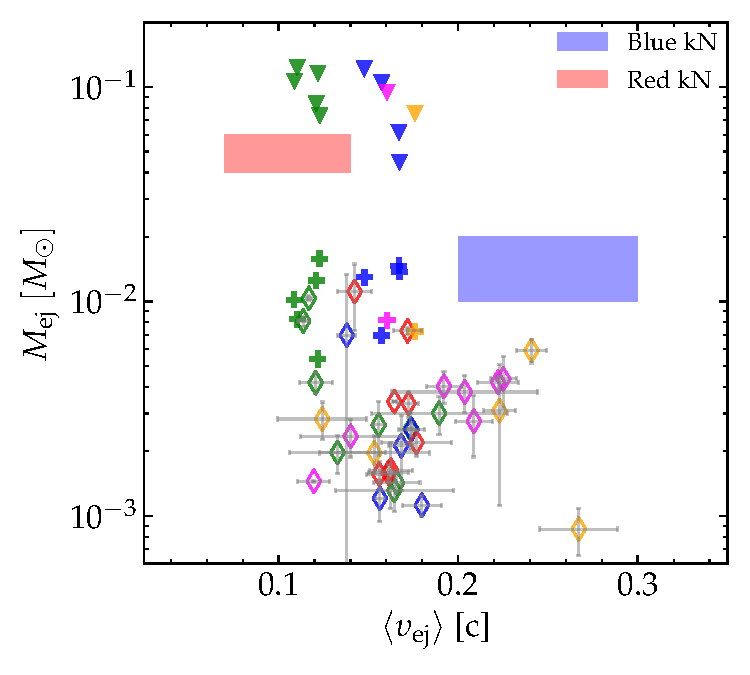
\includegraphics[width=0.48\textwidth]{ejecta_dyn/summary/ej_mej_vej_our2.pdf}
    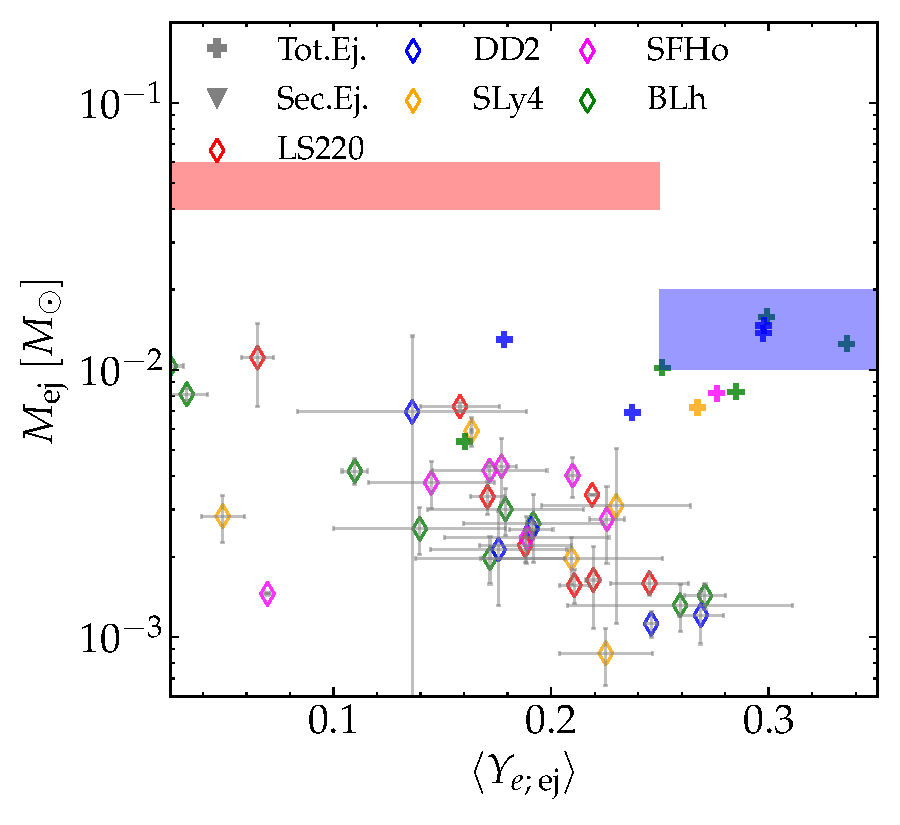
\includegraphics[width=0.48\textwidth]{ejecta_dyn/summary/ej_mej_yeej_our2.pdf}
    \caption{
        Properties of various types of ejecta (indicated with different markers) 
        for all our simulations, alongside the regions inferred for \AT{} 
        (colored patches) based on \citet{Siegel:2019mlp}. 
        %
        Ejecta types shown: \ac{DE} (diamond markers with error bars), 
        \ac{DE} plus \ac{SWW} (solid cross markers), 
        estimated secular ejecta assuming $40\%$ of the disk mass 
        is unbounded on secular timescales with the velocity of \ac{SWW} 
        (down triangle markers).
        %
        (Adapted from \citet{Nedora:2020pak}).
        %        
        %        Summary of the ejecta properties of our models.
        %        %
        %        Diamonds mark the dynamical ejecta, crosses include the
        %        contribution of the \swind{} for the long-lived models, 
        %        triangles are an estimate of the total ejecta mass on a secular
        %        timescale, assuming $40\%$ of the disk mass is unbounded on
        %        secular timescales.         
        %        The ejecta mass is shown is terms of the mass-averaged velocity
        %        (left) and of the averaged electron fraction (right).
        %        %
        %        The filled blue and red patches are the expected values of
        %        ejecta mass and velocity for blue and red components of
        %        AT2017gfo compiled by \cite{Siegel:2019mlp}, based on
        %        \cite{Villar:2017wcc}. 
        %        Adopted from \citet{Nedora:2020pak}.
    }
    %
    \label{fig:ejecta:dyn:ds_sww}
\end{figure*}

In Fig.~\ref{fig:mkn_example} we show the result of our analysis. For clarity we 
show the differences, $\Delta t_{\rm peak} = t_{\rm peak; NR} - t_{\rm peak; fit}$, 
and $\Delta m_{\rm peak} = m_{\rm peak; NR} - m_{\rm peak; fit}$, for peak times, 
$t_p$, and magnitudes, $m_{\rm AB}$, respectively. 
The comparison is shown for $3$ different photometric bands, 
$g$, $z$, and $K_s$ (indicated by different markers) 
and for a set of representative \ac{BNS} merger simulations.

Considering one-component \ac{kN} \acp{LC}, (top panel), we observe 
that the $t_p$ is recovered with an error margin of ${\sim}0.2\,$days 
in $g$ and $z$ bands, and within a $0.5\,$day margin in $K_s$ band. 
Notably, fit-informed \acp{LC} systematically underestimate $t_p$ in the 
$K_s$ band. 
%
The largest deviation is found for the 
model with $q=1.8$ and BLh \ac{EOS}. This highlights a limitation of our 
fitting formula, insofar as it is not able to reproduce \ac{PC} model properties well.

Comparing peak magnitudes, $m_{\rm AB}$, we observe that differences 
between \ac{NR}- and fit-informed \acp{LC} are on average ${\sim}0.5$~mag. 
In $g$ band, however, the deviations are ${\sim}1\,$mag.
Considering two-component \ac{kN} models, we observe that the 
$t_p$ in $K_s$ band differ between the fit- and \ac{NR}-informed \acp{LC} by 
${\sim}2\,$days. The $m_{\rm AB}$ is reproduced within ${\pm}0.5\,$mag 
on average in $z$ and $K_s$ bands.
%
The larger differences in $m_{\rm AB}$ for one component \ac{kN} \acp{LC} 
can be attributed to the influence of the ejecta geometry that is not 
fully accounted for by the  single parameter, $\athetarms$, that we use to 
separate low and high opacity material. 

Overall we observe that, while there are considerable deviations between fit- and 
\ac{NR}-informed \acp{LC} which can be attributed to the limitations of 
our fitting formula as well as the specifics of the \ac{kN} model used for the 
analysis, certain \ac{kN} properties, \eg, peak time in high-frequency bands, 
appear to be captured robustly. 

%Overall, we note that while the exact reasons for deviations can be attributed to 
%the exact \ac{LC} model employed, this example suggests that the minimum systematic 
%variations that are to be expected in synthetic \acp{LC} 
%informed by our best fitting formulae.



%% -----------------------------
%% 
%% -----------------------------

\section{Summary of ejecta kilonova signatures}\label{sec:kilonova:summary}




%% from main paper, referencing the fitpaper Poly22 fits and SWW + DE
%\red{THis can be augmented with Radio afterglow}

%% === FROM DYNAMICAL EJECTA SECTION of MAIN PAPER
%Here we discuss the application of our results to \GW{}.


%\subsection{Dynamical Ejecta}

%In Chapter~\ref{ch:bns_sims}, Sec~\ref{}

%The properties of the dynamical ejecta from the \ac{BNS} mergers are of key 
%importance to determine the properties of the \ac{EM} counterpart. 
%%



Observed data for \AT{} has been extensively studied, and many \ac{kN} models, most of which were spherical, two-component \ac{kN} models, 
were employed to infer the properties of ejecta that produced the observed 
emission \citep[\eg][]{Villar:2017wcc}. 
%
Due to differences in physics input and modeling techniques, these methods gave 
broad ranges of expected values for ejecta mass, velocity and composition 
that read \citep{Siegel:2019mlp}:
%
$M_{\text{ej}}^{\text{red}}\in(4, 6)\times10^{-2}\,\Msun$ and
$\upsilon_{\text{ej}}^{\text{red}}\in(0.07, 0.14)\,c$ for the red component, and 
$M_{\text{ej}}^{\text{blue}}\in(1, 2)\times10^{-2}\,\Msun$ and 
$\upsilon_{\text{ej}}^{\text{blue}}\in(0.2, 0.3)\,c$ for the blue component.
%
We show these ranges in Fig.~\ref{fig:ejecta:dyn:ds_sww}, alongside the 
ejecta properties from our models. 


With respect to the red component, we observe that \ac{DE} from our models 
have too high average velocities and not nearly enough mass.
This result suggests that an additional, low $Y_e$ ejecta component 
is required in order to explain the \AT{} red component 
\citep[\eg][]{Perego:2017wtu,Kawaguchi:2018ptg}.
%

As we showed in Chapter~\ref{ch:bns_sims}, Sec~\ref{sec:bns_sims:dyn}, 
\ac{DE} properties can be mapped onto binary parameters, \eg, 
\mr, $q$, and tidal deformability, $\tilde{\Lambda}$, via a simple 
2nd order polynomial, \polql{}. 
%
The ranges in $q$ and $\tilde{\Lambda}$ inferred for \GW{} from \ac{GW} analysis 
\citep{TheLIGOScientific:2017qsa,Abbott:2018wiz,De:2018uhw,Abbott:2018exr}, 
\ie,  $90\%$ credible intervals, are 
$\tilde{\Lambda}=300_{-190}^{+500}$ and $q\in[1., 1.37]$. 
%
Mapping them onto ejecta parameters via \polql{}, we obtain 
%
$\amd \in [0.72, 7.52] \times 10^{-3}\, \Msun$
and
$\avd \in [0.16, 0.39]\, c$
and 
$\ayd \in [0.11, 0.23]$.
%
Predictably, we observe that the obtained ranges do not agree with those 
inferred for \AT{}. 
This is partially due to the simplified ejecta 
geometry considered in many \ac{kN} models, but also because other 
ejecta types besides \ac{DE} contributed to the observed emission.

% when spherical, two-component \ac{kN} models are 
%considered \citep{Villar:2017wcc}.
%
%Overall, we note that (i) other ejecta components are required to 
%explain the red component of \AT{} and (ii) the non-trivial geometry of 
%\ac{DE} ought to be taken into account in \ac{kN} modeling.


%The analysis of the \ac{kN} non-thermal afterglow, cannot provide conclusive 
%constraints on the properties of \ac{DE} yet. 
%We can only note, that as the mild ejecta velocities seem to be preferred by the 
%emerging new \GRB{} afterglow component, the emitting material had previously 
%contributed to the red component of the \ac{kN} primarily. Such ejecta of 
%mild velocities is found in \ac{BNS} merger simulations with moderately stiff 
%\acp{EOS} and \mr{}s ${\leq}1.8$. 
%%
%Significantly more observational data is required for linking the \ac{kN} and 
%its afterglow to ejecta properties and ultimately to the properties of the 
%binary. 





%\subsection{Spiral-wave wind}

%Discussing the \ac{BNS} models' merger dynamics and outflowing matter we 
%identified a new ejecta component, driven by interactions between the \ac{NS} 
%merger remnant and the disk, \ac{SWW}. % (Ch.~\ref{ch:bns_sims}, Sec.~\ref{sec:bns_sims:dyn}).
%%
%We showed that this ejecta is more massive than \ac{DE} if the \ac{NS} remnant 
%is long-lived, and has high electron fraction. % (Sec.~\ref{sec:bns_sims:sww}).
%
As we showed in Sec.~\ref{sec:kilonova:result}, \ac{SWW} could be 
a significant contributor to \AT{}, assuming that 
the \pmerg{} remnant of \GW{} survived for $\mathcal{O}(100)\,$ms.
Specifically, we showed that \ac{SWW} properties are in line with 
those required to explain the early blue emission of \AT{}. 
%in Ch.~\ref{ch:kilonova}, Sec.~\ref{sec:kilonova:result}.
%
Indeed, as we show in Fig.~\ref{fig:ejecta:dyn:ds_sww} (left panel),
% we show the total ejecta properties 
%(\ac{DE}+\ac{SWW}) for simulations with long-lived \ac{NS} remnants. 
%
the total ejecta (\ac{DE}+\ac{SWW}) mass from several of our models, \eg, 
BLh $q=1.18$, BLh $q=1.42$ and DD2 $q=1.00$ 
is sufficiently massive and proton-rich to account for the blue 
\ac{kN} of \AT{}. Meanwhile, the left panel of Fig.~\ref{fig:ejecta:dyn:ds_sww} 
shows that the total ejecta is slower than what is required. 
%
Notably, ejecta properties inferred from \AT{} change when sophisticated 
radiation transport models, which take into account ejecta geometry and cross-ejecta 
interactions, are considered. Furthermore, other proton-rich ejecta components are 
expected on timescales larger than our simulations permit 
\citep[\eg][]{Fujibayashi:2017puw,Fernandez:2018kax,Radice:2018xqa}.

% in agreement 
%with the expected values for the blue component of \AT{}. 
%%(obtained using the two-component fit \citep{Villar:2017wcc})
%
%The high electron fraction of the \ac{SWW} %(see Sec.~\ref{sec:bns_sims:sww}) 
%however would result in a lanthanides-poor composition of the outflow 
%(Sec.~\ref{sec:nucleo:results}). Thus, the \ac{SWW} cannot explain the 
%observed emission for the high opacity, lanthanides-rich material.
%%
%Simulations with advanced physics of a \ac{MNS} mergers on a timescales 
%${>}100\,$ms are required to asses the contribution from other outflow mechanisms, 
%\citep{Lee:2009uc,Fernandez:2015use,Siegel:2017nub,Fujibayashi:2017puw,Fernandez:2018kax,Radice:2018xqa}.



%\subsection{Secular Ejecta}
%On even longer timescales, 
%On the timescale of seconds, much longer than the evolution of our simulations, 
%nuclear recombination can unbind a fraction of the disk.  
%(See Sec.~\ref{sec:bns_sims:mj_loss} for more details). % See Mb-J plot for example
%

Nuclear recombination and viscous processes are expected to unbind 
${\sim}40\%$ of a disk in a form of outflows with typical velocity 
${\lesssim}0.1\,c$ on a secular timescale 
\citep[\eg][]{Siegel:2017nub,Fujibayashi:2017puw,Fernandez:2018kax,
    Radice:2018xqa,Fujibayashi:2020dvr}. 
%
%Analytical estimates and simulations with various approximations show that 
%up tp ${\sim}40\%$ of the disk can be ejected via viscous processes with an 
%typical velocity ${\lesssim}0.1\,c$ 
%\citep[\eg][]{Siegel:2017nub,Fujibayashi:2017puw,Fernandez:2018kax,
%    Radice:2018xqa,Fujibayashi:2020dvr}. 
%
Considering disk masses of our \ac{BNS} merger simulations and 
adapting the fix fraction of $40\%$ of the $M_{\rm disk}$, we estimate 
that about ${\sim}0.05\, \Msun$ would be ejected in the form of secular winds. 
%
Plotting the expected masses of secular ejecta from our models with long-lived 
remnants (lower triangles in Fig.~\ref{fig:ejecta:dyn:ds_sww}), 
we observe that they would be sufficient to explain the red component of \AT{}. 


A more quantitative analysis requires ab-initio \ac{BNS} merger simulations, 
that are sufficiently long and have sufficiently advanced physics input, to 
capture all the aforementioned ejection mechanisms. 








%% ---------------------
%Sources with time delay are preferred by studies of very metal poor stars that indluded the time delay for r-process elements
%to diffuse through ISM, \citep{Tarumi:2021xvw}. 
%A winds from proto-nuetron are also contributors to the $r$-process budget \cite{Vincenzo:2021rvw}
%
%\red{The remnant is losing anular momentum while disk gains on shortly after merger is due to gravitational torque \cite{Shibata:2019wef}}
%




